\documentclass[tikz]{standalone}
\usepackage{circuitikz}
\begin{document}


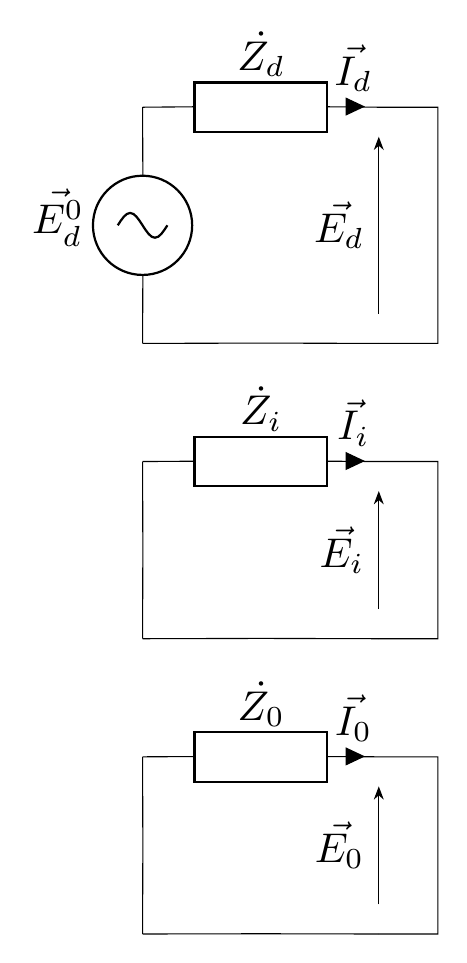
\begin{tikzpicture}[scale=1.5, transform shape]
\draw (10.5,9.5) to[european resistor,l=$\dot{Z_0}$,i=$\vec{I_0}$] (12.5,9.5) -| ++(0.5,0)  |- ++(-0.5,-1.5);
\draw (10.5,13) to[sinusoidal voltage source,l=$\vec{E_d^0}$] (10.5,15);
\draw (10.5,15) to[european resistor,l=$\dot{Z_d}$,i=$\vec{I_d}$] (12.5,15) -| ++(0.5,0)  |- ++(-0.5,-2) ;
\draw (10.5,12) to[european resistor,l=$\dot{Z_i}$,i=$\vec{I_i}$] (12.5,12) -| ++(0.5,0)  |- ++(-0.5,-1.5);
\draw (10.5,13) to[short] (12.5,13);
\draw (10.5,12) to[short] (10.5,10.5);
\draw (10.5,10.5) to[short] (12.5,10.5);
\draw (10.5,9.5) to[short] (10.5,8);
\draw (10.5,8) to[short] (12.5,8);
\draw [->, >=Stealth] (12.5,13.25) -- (12.5,14.75)node[pos=0.5,anchor=east]{$\vec{E_d}$};
\draw [->, >=Stealth] (12.5,10.75) -- (12.5,11.75)node[pos=0.5,anchor=east]{$\vec{E_i}$};
\draw [->, >=Stealth] (12.5,8.25) -- (12.5,9.25)node[pos=0.5,anchor=east]{$\vec{E_0}$};
\end{tikzpicture}


\end{document}
